\begin{center}
    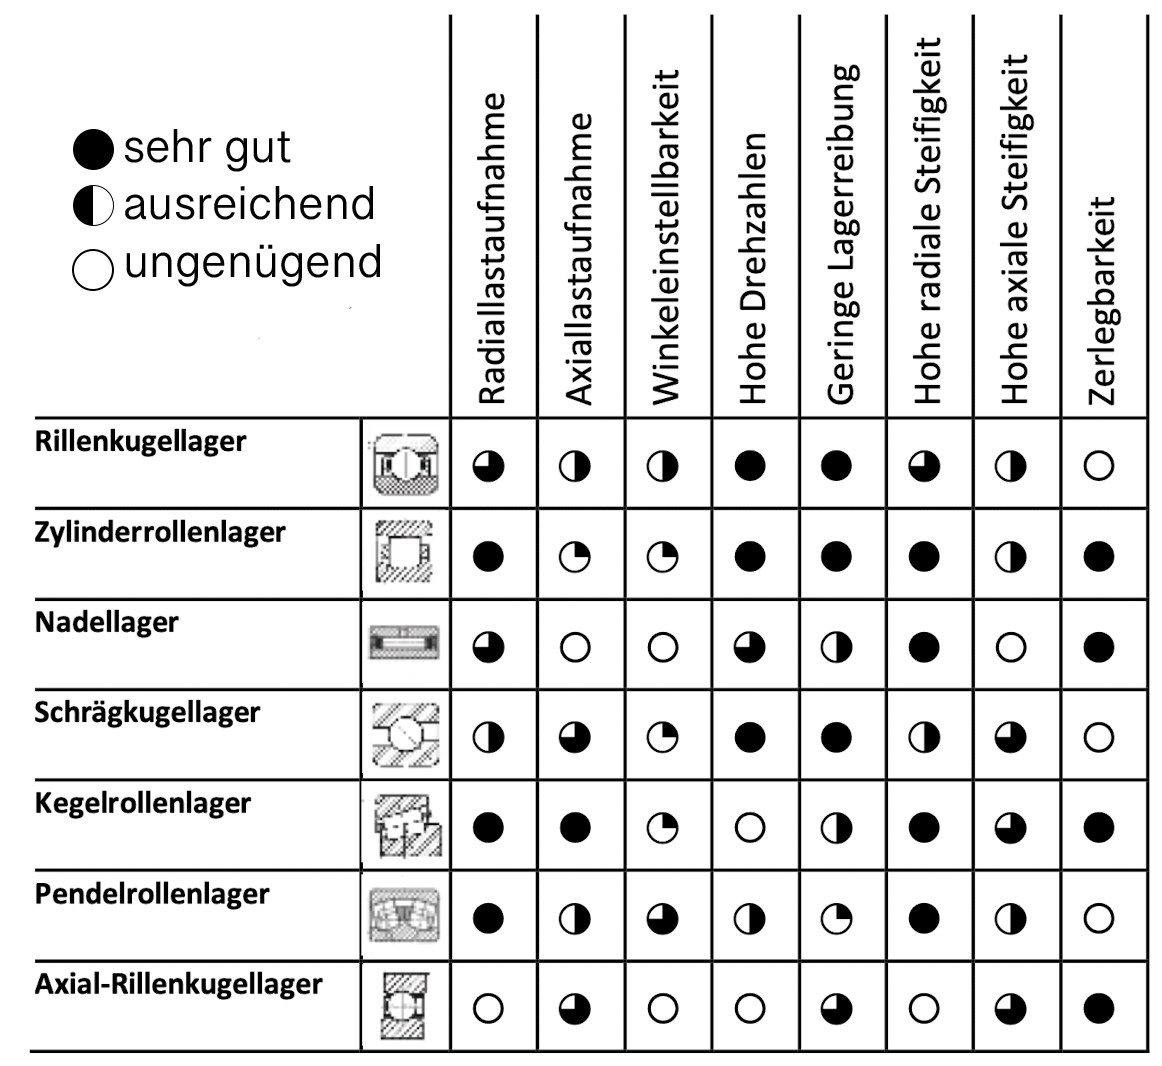
\includegraphics[width = 0.9\linewidth]{src/images/MAEIP_Lagerungen}
\end{center}
\begin{scriptsize}
    \begin{itemize}
        \item \textbf{Fest-Los:} \underline{Pro:} eindeutige Positionierung / Axialbelastung / Längen-\\ausgleich durch Loslager / statisch bestimmt
        \\ \underline{Contra:} zusätzliche Fertigungsschritte / hohe Kosten
        \item \textbf{Schwimmend:} \underline{Pro:} geringe Kosten / Längenausgleich
        \\ \underline{Contra:} keine wechselnde Axiallasten / schlechte Positionierungsgenauigkeit
        \item \textbf{Angestellt X:} \underline{Pro:} hohe Axialkräfte / hohe Positionierungsgenauigkeit / Kräfte zwischen Lager 
        \\ \underline{Contra:} hohe Kosten / kein Längenausgleich
        \item \textbf{Angestellt O:} \underline{Pro:} hohe Axialkraft / hohe Positionierungsgenauigkeit / Kräfte ausserhalb Lager
        \\ \underline{Contra:} hohe Kosten / kein Längenausgleich
        \\~\\
        \item \textbf{Passungswahl:} 
        \\ \textbf{Punktlast:} $\Rightarrow$ Spiel / \textbf{Umfangslast:} $\Rightarrow$ Übermass 
    \end{itemize} 
\end{scriptsize}